% gr-Hanoi.tex -- the Sierpinski graph S(4,3), isomorphic to the graph of
% the Tower of Hanoi with 4 discs (81 states, 120 moves).
% A vertex d1d2d3d4 is placed at the sum of the corners c(dk) scaled by
% L^(4-k) ; u = s i j..j ~ v = s j i..i. The bottom side, from 0000 to
% 2222, is an optimal solution : 15 moves, the words of {0,2}^4 in the
% order of the binary numbers. Engine : pdfLaTeX or LuaLaTeX
\documentclass[border=3mm, convert=false]{standalone}
\usepackage{tkz-berge}
\begin{document}
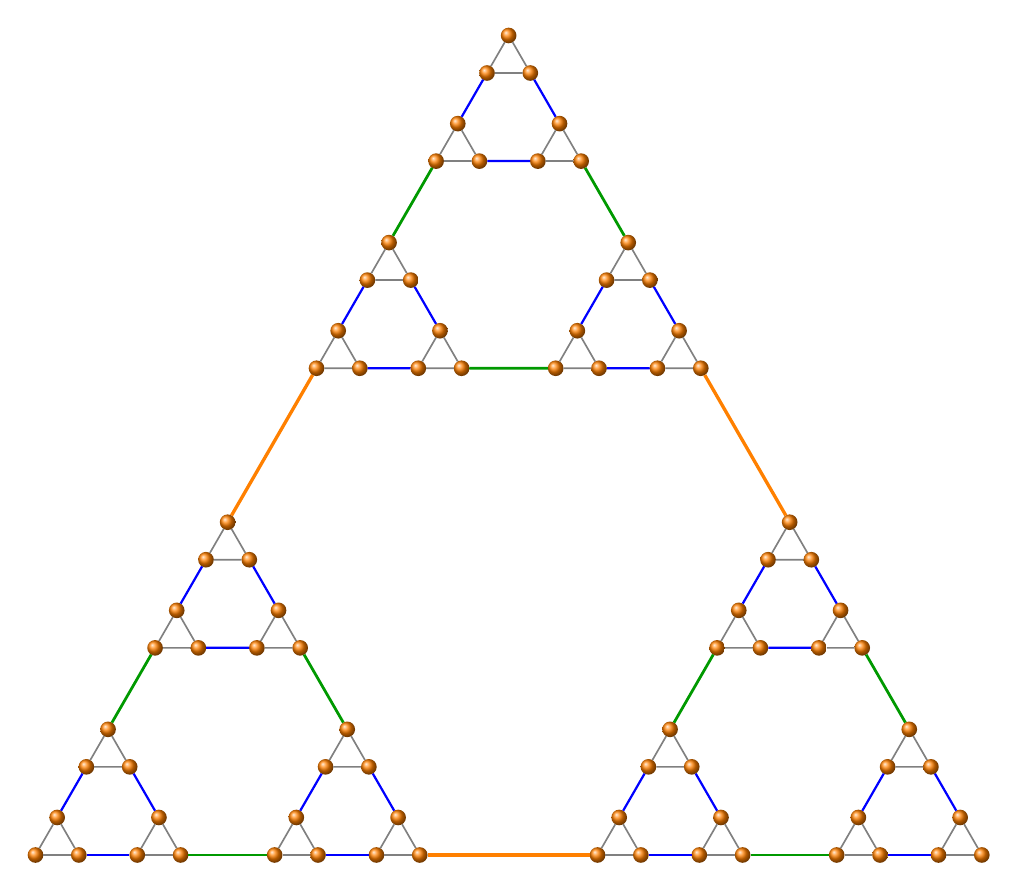
\begin{tikzpicture}[scale=.55]
  \GraphInit[vstyle=Art]
  \SetVertexNoLabel
  \tikzset{VertexStyle/.append style = {minimum size = 5pt}}
  \def\L{2.35}
  \def\cx{{0,0.5,1}}\def\cy{{0,0.866,0}}
  \foreach \a in {0,1,2}{\foreach \b in {0,1,2}{%
  \foreach \c in {0,1,2}{\foreach \d in {0,1,2}{%
    \pgfmathsetmacro\x{\cx[\a]*\L^3+\cx[\b]*\L^2+\cx[\c]*\L+\cx[\d]}
    \pgfmathsetmacro\y{\cy[\a]*\L^3+\cy[\b]*\L^2+\cy[\c]*\L+\cy[\d]}
    \Vertex[x=\x,y=\y]{\a\b\c\d}}}}}
  \foreach \i/\j in {0/1,0/2,1/2}{%
    % moves of the smallest disc
    \foreach \a in {0,1,2}{\foreach \b in {0,1,2}{\foreach \c in {0,1,2}{%
      \Edge[local,color=gray,lw=.6pt](\a\b\c\i)(\a\b\c\j)}}}
    % the other discs
    \foreach \a in {0,1,2}{\foreach \b in {0,1,2}{%
      \Edge[local,color=blue,lw=.8pt](\a\b\i\j)(\a\b\j\i)}}
    \foreach \a in {0,1,2}{%
      \Edge[local,color=green!60!black,lw=1pt](\a\i\j\j)(\a\j\i\i)}
    \Edge[local,color=orange,lw=1.2pt](\i\j\j\j)(\j\i\i\i)}
  \tkzHighlightPath[color=red,lw=2.5pt,style={opacity=.6}]%
    {0000,0002,0020,0022,0200,0202,0220,0222,
     2000,2002,2020,2022,2200,2202,2220,2222}
\end{tikzpicture}
\end{document}
